\section{Discussion}
\label{sec:flakycat-discussion}

\subsection{Reasoning about the statements influencing FlakyCat and the usage of flakiness categories}
\label{sec:discussion:reasoning}

Listing~\ref{lst:flaky-example} gives an example of a flaky test taken from the Neo4J project\footnote{https://github.com/neo4j/neo4j/commit/c77e579b40b02087} found during the data collection part.
As explained in the commit message, the flakiness was caused by a race condition and thus, we affected it to the Concurrency category. FlakyCat classified this test as Async wait. The interpretability technique that we introduced in Section~\ref{sec:flakycat-interpretability} reveals that the statement on line 6 is the most influential for the model's decision. It contains the \texttt{await()} function, and this is likely the reason why the flaky test was categorized as Async wait. Furthermore, similarity score for the Concurrency category is high, and it comes as FlakyCat's second guess. 

When looking at the test, we understand that an asynchronous wait was performed to wait for a thread. We also found similar examples concerning other categories, such as waits relying on network resources. First, we argue that our interpretability technique can help to understand the cause of flakiness, even when FlakyCat apparently mislabelled the test. Secondly, we advance that flakiness categories as commonly defined in research studies~\cite{Luo2014, Eck2019} can overlap, \ie a flaky test can belong to several categories. The application of machine learning to determine the causes of flakiness is promising and should receive attention. It would also benefit from a more precise, orthogonal classification of flakiness categories. \\


\begin{lstlisting}[caption={A flaky test belonging to two categories
},label={lst:flaky-example},language=Java]
@Test
public void shouldPickANewServer[...]() throws Throwable {
[...]
    Thread thread = new Thread( () -> {
    try {
    startTheLeaderSwitching.await();
    CoreClusterMember theLeader = cluster.
        awaitLeader();
    switchLeader( theLeader );
    } catch ( TimeoutException | InterruptedException e ) {
        // ignore
    }});
[...]
}
\end{lstlisting}

\subsection{The effect of considering an additional category}
Our results showed that flakiness categories can be classified automatically. We carried out our main experiments with five categories of flakiness for which we had a reasonable number of tests. Still, we believe that one interesting aspect of our study is to understand the impact of adding other categories to FlakyCat. 
For this, we investigate the performance of FlakyCat for each category (similarly to RQ2), but we add to our set the \textit{Network} category,
which is the next category with the most samples in our dataset (25 tests). F1 scores and the accuracy obtained for each category are presented in Figure \ref{fig:fsl_add_class}. 

Compared to the results previously reported in Table~\ref{scores}, we observe that the performances of each category are slightly impacted.
The \textit{Async waits} category is the most impacted one. 
Indeed, after adding the \textit{Network} category, we get an overall F1 score of 0.68. The added category gets the worst results. 
This performance drop can be explained by multiple factors.
First, having more categories to differentiate makes it more challenging for FlakyCat to distinguish between them.
Secondly, the overall F1 score is strongly affected by the poor performance observed in the new category.
The performance for the Network category can be a result of the too low number of examples in this category (25). Despite using FSL, the model still requires enough data points in each category. While collecting data, we noticed that flaky tests caused by Network were not common. These findings align with the ones about the prevalence of the different categories reported in previous empirical studies~\cite{Luo2014,Eck2019}. In addition, flaky tests related to \textit{Network} issues could also be considered as Asynchronous waits in many cases, as previously explained. 


\begin{figure}[htbp]
\centering
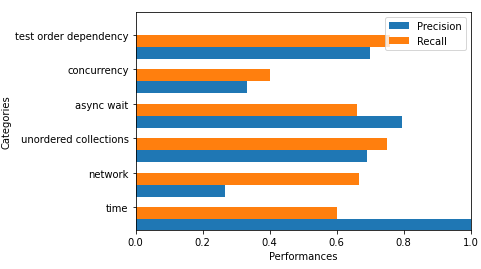
\includegraphics[scale=0.8]{figures/flakycat/add_network.PNG}
\caption{Precision and Recall per flakiness category when adding the category "Network" }
\label{fig:fsl_add_class}
\end{figure}